\documentclass[a4paper,10pt]{article}
\usepackage[utf8]{inputenc}

\usepackage{amsmath} 
% \usepackage[T1]{fontenc}
\usepackage{graphicx}
%\documentclass{article}
%\usepackage[showframe]{geometry}
\usepackage{layout}
\usepackage[margin=.75in]{geometry}
%\usepackage{multirow}
\usepackage{hhline} %for double hlines
\usepackage{booktabs} %for all professional-looking table characterictics ;-)
\usepackage{float}
\restylefloat{table}
\floatstyle{plaintop}
\usepackage[tableposition=top]{caption}
\renewcommand{\arraystretch}{1.5}

\usepackage{subcaption}
\usepackage{xcolor}
\usepackage{listings}
\usepackage{caption}
\DeclareCaptionFont{white}{\color{white}}
\DeclareCaptionFormat{listing}{%
  \parbox{\textwidth}{\colorbox{gray}{\parbox{\textwidth}{#1#2#3}}\vskip-4pt}}
\captionsetup[lstlisting]{format=listing,labelfont=white,textfont=white}
% \lstset{frame=lrb,xleftmargin=\fboxsep,xrightmargin=-\fboxsep}

\lstset{language=Python, showspaces=false, showstringspaces=false, numbers=None, breaklines=true}

\usepackage{epigraph}

% Title Page
\title{\textbf{Python in the enterprise} \\ Machine-learning-based silicon sensor quality evaluation}
\author{Dawid Gerstel, Marcin Lis, Michał Łabuz, Konrad Zuchniak}

\begin{document}
\maketitle


% \epigraph{No amount of experimentation can ever prove me right; a single experiment can prove me wrong.}{\textit{Albert Einstein}}

\newpage

\section{Introduction}

The goal was to implement software for classifying silicon sensors as either good or bad ones. The k-nearest neighbours algorithm was to be used to assess a sensor's response 
based upon a few attributes in the so-called feature space. These, in turn, were to be obtained in a preprocessing from sensor's response histograms in the ROOT framework. This report summarises the project functionality, evolution, methodology used and results obtained.

\section{Managing the project}
At the beginning, the tasks were assigned to the authors of this report as follows:

\begin{table}[H]
\centering
\begin{tabular}{@{}lc@{}} \toprule %\cline{3-6}
\multicolumn{1}{c}{task}& person responsible \\ \toprule
Analysis of the sensor's response histograms & all \\
Choosing specific ML algorithm & all \\
Histograming the measurements in the feature space & Dawid G. \\
Extracting feature space attributes from the histograms & Dawid G. \\
ML algorithm implementation & Michał Ł. \& Konrad Z. \\
Testing accuracy of the algorithm & all \\
Implementing graphical user interface & Marcin L. \\
Results analysis & all \\
Functionality testing and suggesting improvements & all
\bottomrule
\end{tabular}
\caption{Summary of the tasks assigned to the team members at the project's start}
\label{t:tasks}
\end{table}


Naturally, the team did not strictly respect the above task division as oftentimes authors asked and helped each other rather spontaneously.
The team used git repository and the project is accessible at \url{https://github.com/dgerstel/PITE-Sensor-Eval}.

\section{Project overview -- its evolution and dataflow}

The input data come from the real silicon sensors of the LHCb's Vertex Locator. There are 42 sensors in total and each one has 2048 channels at which noise (with pedestal subtracted) had been observed producing 2-dimensional histograms as in the Fig. \ref{f:2D}. We had been supplied with these data
\newline (\texttt{.../data/165526/VELODQM\_165526\_2015-10-12\_18.05.29\_NZS.root}) before the project started. Then, we created a ROOT macro \texttt{.../code/preprocessData.C} 
that scanned over the ROOT file, extracted the 2-dimensional distributions and projected them onto y-axis building 1-dimensional sensor noise distributions that are irrespective of its channels. Fig. \ref{f:1D} shows an exemplary such plot.
Both types of histograms are saved in \texttt{.../fig/control\_plots/}.


\begin{figure}[H]
    \centering
    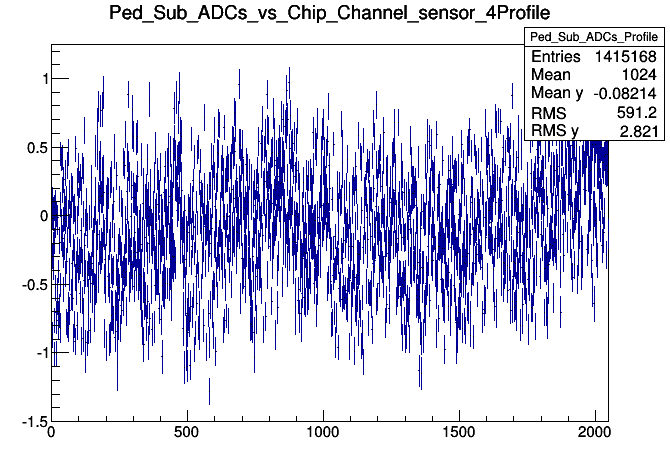
\includegraphics[width=.7\textwidth]{../fig/control_plots/sample_ADC_vs_chann}
    \caption{Mean noise after pedestal substraction (y-axis) for subsequent channels (x-axis).}
    \label{f:2D}
\end{figure}

\begin{figure}[H]
    \centering
    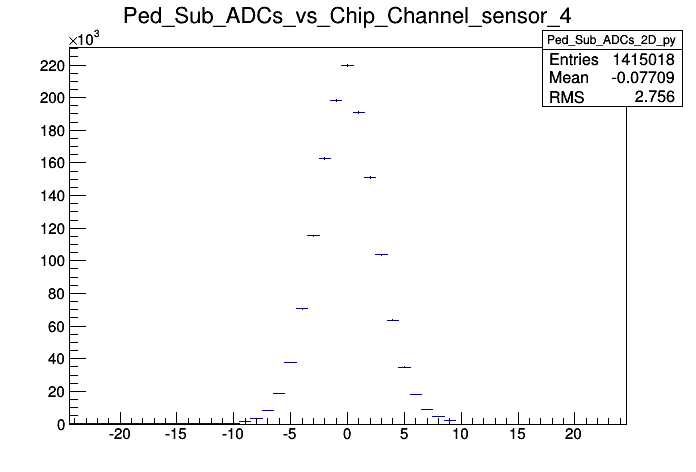
\includegraphics[width=.7\textwidth]{../fig/control_plots/sample_ADC_distr}
    \caption{Frequency distribution of mean noise (x-axis).}
    \label{f:1D}
\end{figure}


Then, from these distributions four parameters were extracted, namely: mean, rms, skewness and kurtosis. These comprised the attributes for a machine learning algorithm. For any supervised learning it is mandatory to provide an adequate class label. We decided to approach classification as binary (either good or bad) with a perspective to develop a continuous and probabilistic classification to either category later on (if at all).
The resulting data are stored in \texttt{.../data/sensorData.dat}.


After a brief analysis by eye we agreed that all 42 sensors are acceptable and we attributed them class '1' (good).


Next, because we were supplied with only good sensors -- we had to simulate response of low-quality ones by shifting attributes of the 'good' ones. It is done by a function in \texttt{FakeData.py} ...
The simulated low-quality sensor results are stored in files with prefix \texttt{.../data/danefake*}.

Then, we implemented k-nearest neighbours classifier (\texttt{.../code/Classifier.py}), taught the algorithm using the real sensor and simulated samples and, finally, we tested the classification accuracy. To this end, we used k-fold cross-validation described in the next section.



% To make the algorithm more useful a probabilistic approach needs to be taken in which a percentage that a given sensor is acceptable is inferred.
% \footnote{This objective is, unfortunately, beyond the scope of the knn classifier.}
% To satisfy this requirement we came up with an idea of deriving quality estimate (0-100 \% range) based on a sensor's distance (in the feature space) from the most representative one -- so-called the benchmark sensor -- which could simply be represented by averaging all attributes of all good sensors dataset.

% % % However, in due course, we have discovered the logistic regression classifier that yields probabilities of an instance's membership to given classes.

\section{Methodology}
Below we describe classes and functions used that come from the scikit-learn library\footnote{\url{http://scikit-learn.org/stable/}}.

\textbf{\texttt{KNeighborsClassifier}} is a class for classification based on nearest neighbours and it provides instance-based learning, as it does not attempt to construct
a general internal model, but simply stores instances of the training data. Class constructor takes parameters as below:
\begin{lstlisting}
	class sklearn.neighbors.KNeighborsClassifier(n_neighbors=5, weights='uniform', algorithm='auto', leaf_size=30, p=2, metric='minkowski', metric_params=None, n_jobs=1, **kwargs)
\end{lstlisting}


In this small project we used only a few of them:
\begin{itemize}
    \item \texttt{n\_neighbors} is the number of nearest neighbors which should be taken under consideration;
    \item \texttt{weights} parameter has two choices: ‘uniform‘ and ‘distance‘. For the ‘uniform‘ weight, each of the k neighbours has equal vote whatever its distance from the target point is. 'distance' weights points by the inverse of their distance. \texttt{weight} may also be a user defined function;
    \item \texttt{algorithm} parameter lets user to choose which algorithm should be used to compute the nearest neighbours; 'auto' means that class will attempt to decide the most appropriate one itself;
    \item \texttt{metric} decides how distances are calculated in parametric space. A general formulation of distance metric is ‘minkowski’ distance.
\end{itemize}


\texttt{KNeighborsClassifier} methods used in this project:
\begin{itemize}
    \item \texttt{KNeighborsClassifier.fit(X,y)} fits the model using \texttt{X} as training data and \texttt{y} as target values, where \texttt{X} is an array-like object;
    \item \texttt{KNeighborsClassifier.predict(X)} predicts the class labels for the provided data, where \texttt{X} is an array-like object;
    \item \texttt{KNeighborsClassifier.predict\_proba(X)} returns probability estimates for the test data \texttt{X}, where \texttt{X} is an array-like object.
\end{itemize}    
    
To evaluate classification accuracy we used k-fold cross-validation, which is a model validation technique for assessing how the results of a statistical analysis will generalize
to an independent data set. It is mainly used in settings where the goal is prediction, and one wants to estimate how accurately a predictive model will perform in practice. 
The scikit-learn library for cross-validation provides class named \texttt{cross\_validation} which has 2 methods which we used in the project:
\begin{itemize}
  \item \texttt{cross\_validation.ShuffleSplit} random permutation cross-validation iterator. Does not guarantee that all folds will be different. However, this is still very likely for sizeable datasets;
  \item \texttt{cross\_validation.cross\_val\_score} evaluates score by cross-validation.
\end{itemize}

\section{Analysis}
% The tool which we have created, helps us run three independent from each other analysis about sensors' quality. First one tell us something about
% paremeters obained from measurement data by showing histograms of average, RMS, kurtosis and skewness parameters. As we can see in the picture 1
% and 2 (avarege and skewness) there are some significant differences between results.

With the application there are two different types of analyses possible to perform. First of all, we may look at histograms of sensor's noise parameters, like for instance mean and skewness distributions that are depicted in Fig. \ref{f:mean} and Fig. \ref{f:ske}, respectively. The second type allows for evaluating knn algorithm output. Fig. \ref{f:ana} represents classification accuracy as a function of number of neighbours for sample split according to various train-to-test-ratios. This example shows that for splitting the sample into equal halves for training and test we obtained highest -- 100\% -- accuracy.


\begin{figure}[H] \centering
    \includegraphics[width=.8\textwidth]{../fig/app_shots/average}
    \caption{Average parameter histogram.}
    \label{f:mean}
\end{figure}
\begin{figure}[H] \centering
    \includegraphics[width=.8\textwidth]{../fig/app_shots/skewness}
    \caption{Skewness parameter histogram.}
    \label{f:ske}
\end{figure}

\begin{figure}[H] \centering
    \includegraphics[width=.8\textwidth]{../fig/analyse/example}
    \caption{An exemplary analysis plot showing accuracy as a function of number of neighbours for various train-to-test ratios.}
\end{figure}
% This may signal that some sensors should be checked. Second type of analysis is a comparison with benchmark sensor (picture 3).
% \begin{figure}[H] \centering
%     \includegraphics[width=.8\textwidth]{../fig/app_shots/quality}
%     \caption{Comparison to benchmark sensor.}
%     \label{f:ana}
% \end{figure}
% At this point it is important to decide whether some bad quality sensors shouldn't be
% deleted from model as they may cause mistakes in KNN algorithm. The last type of analysis is scoring which give us probability of correct
% data classification.

\section{Summary}
\textit{Python in the enterprise}, as the name suggests, is a subject oriented on utilising Python as a tool for delivering a product of, usually, a team enterprise, whether for business or scientific purposes. The latter motivation characterised this project. Its completion let us develop both --  hard and soft skills. Apart from practising and reviewing the programming language itself, the following traits of team work we would like to emphasise.
First of all, we had to come up with clear division of responsibilities and organisation of working time. Team work made us realise how important reliable code documentation and control of project progress is.
Additionally we understood purpose of using revision control system, like in our case $git$. Some functions in our code were written, at least in part,
by all of us. Thanks to that we could compare the way we think, observe and compare various programming styles and learn something new.

As far as hard skills are concerned, we had a chance to get to know basics of Machine Learning in Python. Particularly well we familiarised ourselves with k nearest neighbours algorithm
and \texttt{KNeighborsClassifier} class from scikit-learn module. To understand classification based on KNN we had to read thoroughly documentation of the class
and learn its methods and attributes.


Finally, we managed to complete all the plans and built models that help distinguish low and high quality silicon sensors based on their noise analysis and machine learning, what is an evidence of our good work organisation.


\appendix
\section{Application guide}

\begin{figure}[H] \centering
    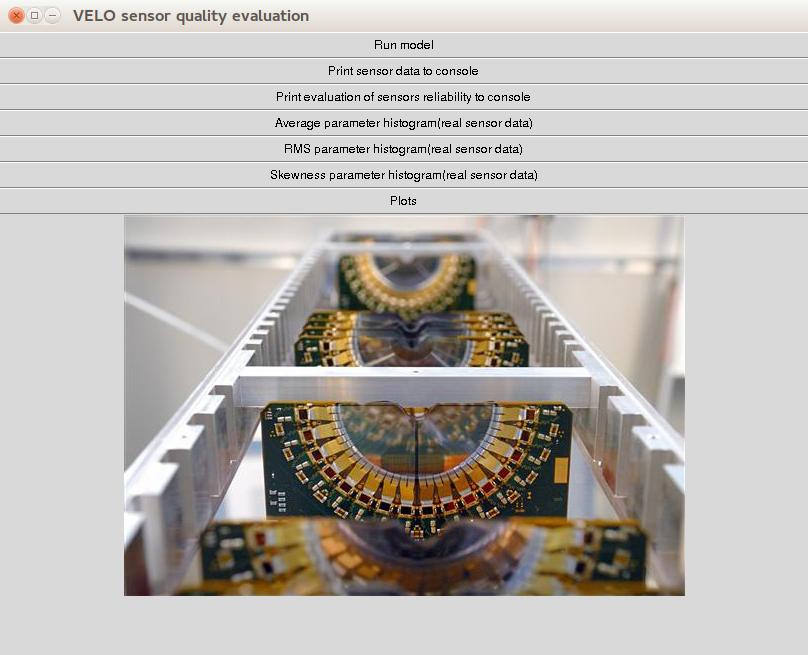
\includegraphics[width=.8\textwidth]{../fig/app_shots/start}
    \caption{Application GUI after start}
\end{figure}

After starting the application with invoking \texttt{python \_\_init\_\_.py} from the directory \texttt{.../code} and clicking \texttt{Start} button the above screen pops up.
\begin{itemize}
    \item \texttt{Run model} -- Enables to run KNN classification of all data from \texttt{.../data} directory; it also allows to generate simulated data.
    \item \texttt{Print sensor data to console} - Displays content of sensor data file with all its parameters and class label.
    \item \texttt{print evaluation of sensors reliable to console} - shows output in console and saves it to the log files.
    \item \texttt{Average/RMS/Skewness parameter histogram} - displays histograms of corresponding parameters of a real sensor.
    \item \texttt{Plots} - Contains analysis plots of accuracy as a function of number of neighbours for various parameter values.
\end{itemize}

\begin{figure}[H] \centering
    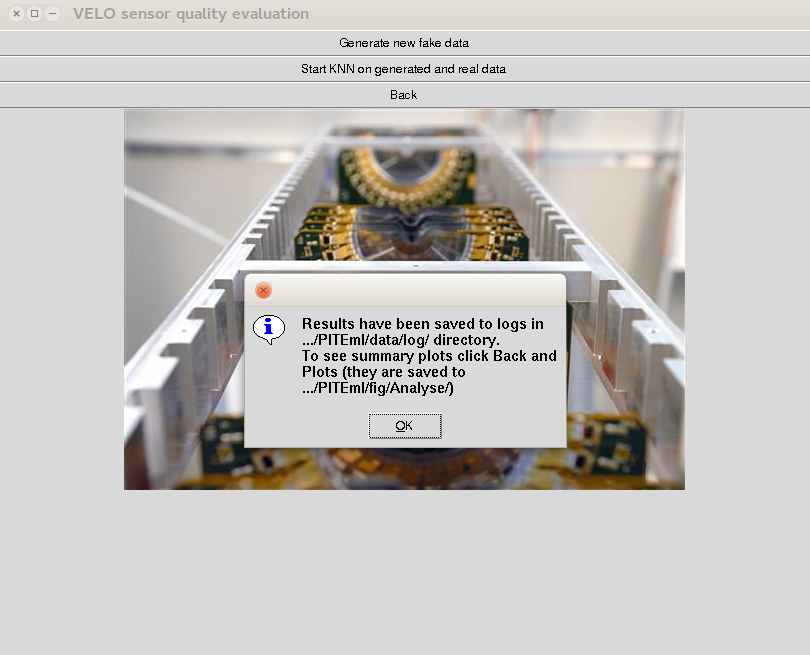
\includegraphics[width=.8\textwidth]{../fig/app_shots/model}
    \caption{Application GUI after choosing \texttt{Run model} from the initial window.}
\end{figure}

\begin{itemize}
    \item \texttt{Generate new fake data} - Generates new simulated sensor data of departure from real sensor parameters as chosen by user.
    \item \texttt{Start KNN on real and generated data} - Launches KNN algorithm and produces output in log files as well as plots.
\end{itemize}


\begin{figure}[H] \centering
    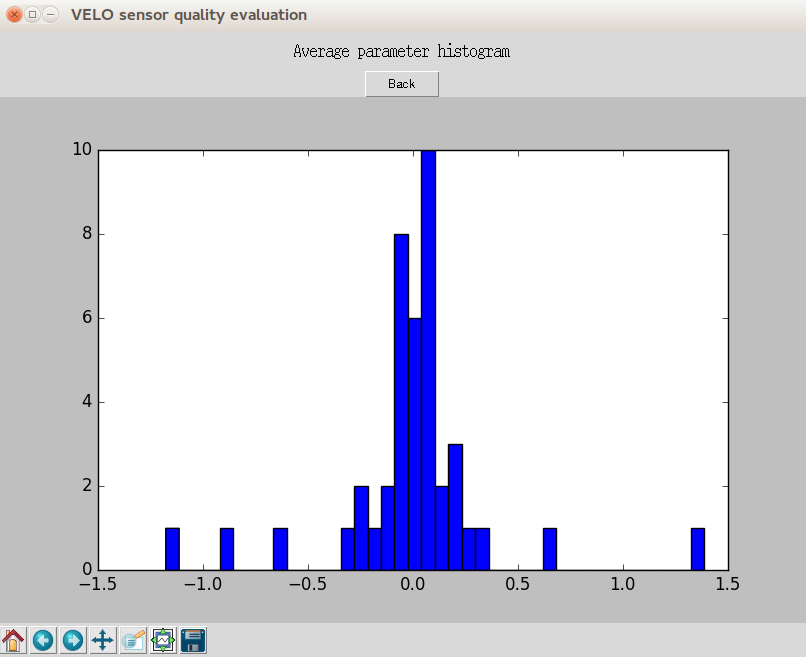
\includegraphics[width=.8\textwidth]{../fig/app_shots/hist}
    \caption{An example of a real sensor histogram.}
\end{figure}

%===== IDEAS ========================
% We concluded that weights 






\end{document}          
